% !TeX root = ./Dyplom.tex

\chapter{Reprezentacja wektorowa}
	W zagadnieniach NLP (ang. \emph{Natural Language Processing}) słowa wyrażone są w postaci wektorów liczb rzeczywistych (ang.\ \emph{word embedding}).
	W powstałej przestrzeni odległość między wektorami reprezentującymi podobne słowa jest mniejsza, niż odległość między słowami o różnym znaczeniu.
	Tradycyjne metody opierają się na semantyce dystrybucyjnej.
	Zgodnie z tą teorią, słowa występujące w podobnym kontekście mają podobne znaczenie.
	Bazując na tej zasadzie skonstruowano wiele algorytmów, zdolnych do wygenerowania wektorów słów analizując dużą ilość nieustrukturyzowanych tekstów.
	Architektura takich modeli opiera się na sieciach neuronowych próbujących przewidzieć słowo w zależności od kontekstu
		(modele CBOW --- ang. \emph{Continuous bag-of-words}) lub kontekst w zależności od słowa (ang.\ \emph{skip-gram})\cite{word2vec}, gdzie kontekst to otaczające słowa.
	Wadą tych modeli jest fakt, że są one niekontekstowe.
	Oznacza to, że po nauczeniu modelu, gdy chcemy go wykorzystać do obliczenia wektora danego słowa, to otrzymany wektor nie bierze pod uwagę kontekstu, w jakim występuje to słowo.
	Przykładowo słowo ,,zamek'' będzie reprezentowane przez taki sam wektor niezależnie od tego,
		czy w danym zdaniu odnosi się do zabezpieczenia antywłamaniowego, czy też widowiskowej dolnośląskiej budowli obronnej.
	
	W 2018 r ukazała się praca prezentująca BERT (ang.\ \emph{Bidirectional Encoder Representations from Transformers})\cite{BERT}.
	Był to pierwszy model kontekstowy.
	Oparty jest na transformerach\cite{Transformers} --- mechanizmach wykorzystujących bloki atencji.
	Mechanizmy te wykrywają zależności między słowami w zdaniu.
	Do warstwy atencji wszystkie słowa wprowadzane są równolegle, a na wyjściu dla każdego słowa otrzymujemy ważoną sumę wektorów wszystkich słów.
	Im większe powiązanie słowa ze słowem analizowanym, tym większa waga.
	Przykład zilustrowany na rysunku~\ref{fig:attention} przedstawia wagi poszczególnych słów w zdaniu ,,The animal didn't cross the street because it was too tired'' w kontekście słowa ,,it''.
	Zaimek ten może odnosić się zarówno do zwierzęcia z początku zdania (ang.\ \emph{The animal}), jak i ulicy (ang.\ \emph{the street}).
	Mechanizm przypisał największą wagę do zwierzęcia, co jest poprawnym działaniem w kontekście tego zdania.
	\begin{figure}[ht]\label{fig:attention}
		\centering
		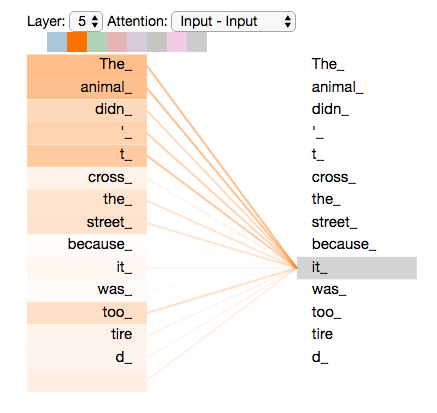
\includegraphics[width=.5\textwidth]{rys03/transformer_attention.png}
		\caption{Mechanizm atencji --- wizualizacja wag poszczególnych słów podczas analizy słowa ,,it''.
			Źródło: https://jalammar.github.io/illustrated-transformer}
	\end{figure}
	
	Równoległe wprowadzanie wszystkich słów wymusza górne ograniczenie na długość zdania.
	Dla większości modeli bazujących na transformerach limit wynosi 512 tokenów.
	Tokenem może być zarówno słowo, jak i część zdania typu przecinek, stąd faktyczny limit liczony w słowach jest jeszcze niższy.
	Jest to mocno ograniczający limit w kontekście wykorzystywanego korpusu, w którym wypowiedzi często złożone są z kilkudziesięciu zdań.
	Problem ten opisywany jest szerzej w rozdziale~\ref{sec:sentences}.

\section{Wektory zdań}
	Modele bazujące na BERT stworzone są z myślą generowania wektorów dla każdego tokena wejściowego.
	Otrzymane w ten sposób wektory kodują informacje semantyczne o wszystkich słowach zdania, jednak nie zawierają informacji o samym zdaniu.
	Jedną z możliwości jest wykorzystanie wartości wektora dla tokena \verb|CLS| --- jest to token wykorzystywany podczas uczenia modelu i reprezentuje znaczenie zdania w kontekście zadań klasyfikacji.
	Można również uśrednić wektory wszystkich słów, jednak nie wszystkie słowa w zdaniu niosą tak samo dużo znaczenia.
	
	Rozwiązanie tego problemu proponują autorzy Sentence-BERT\cite{sbert}.
	Model SBERT złożony jest z dwóch modli BERT połączonych w syjamską sieć.
	Na wyjściu każdego modelu BERT dołożona jest warstwa pooling zwracająca wektor ustalonego rozmiaru dla zdań różnych długości.
	Najlepszą strategią okazała się metoda uśredniania wektorów wszystkich tokenów.
	Następnie wyjściowe dwa wektory wynikowe są łączone i obliczana jest funkcja straty klasyfikatorem \verb|softmax|.
	Architektura ta przedstawiona została na rysunku~\ref{fig:sbert}.
	W celu uzyskania wektorów kodujących semantykę całych zdań, model uczony jest na korpusach zawierających pary zdań oznaczone pod kątem podobieństwa.
	Optymalizuje się odległość między podobnymi zdaniami, jednocześnie maksymalizując odległości między zdaniami różnymi.
	\begin{figure}[ht]\label{fig:sbert}
		\centering
		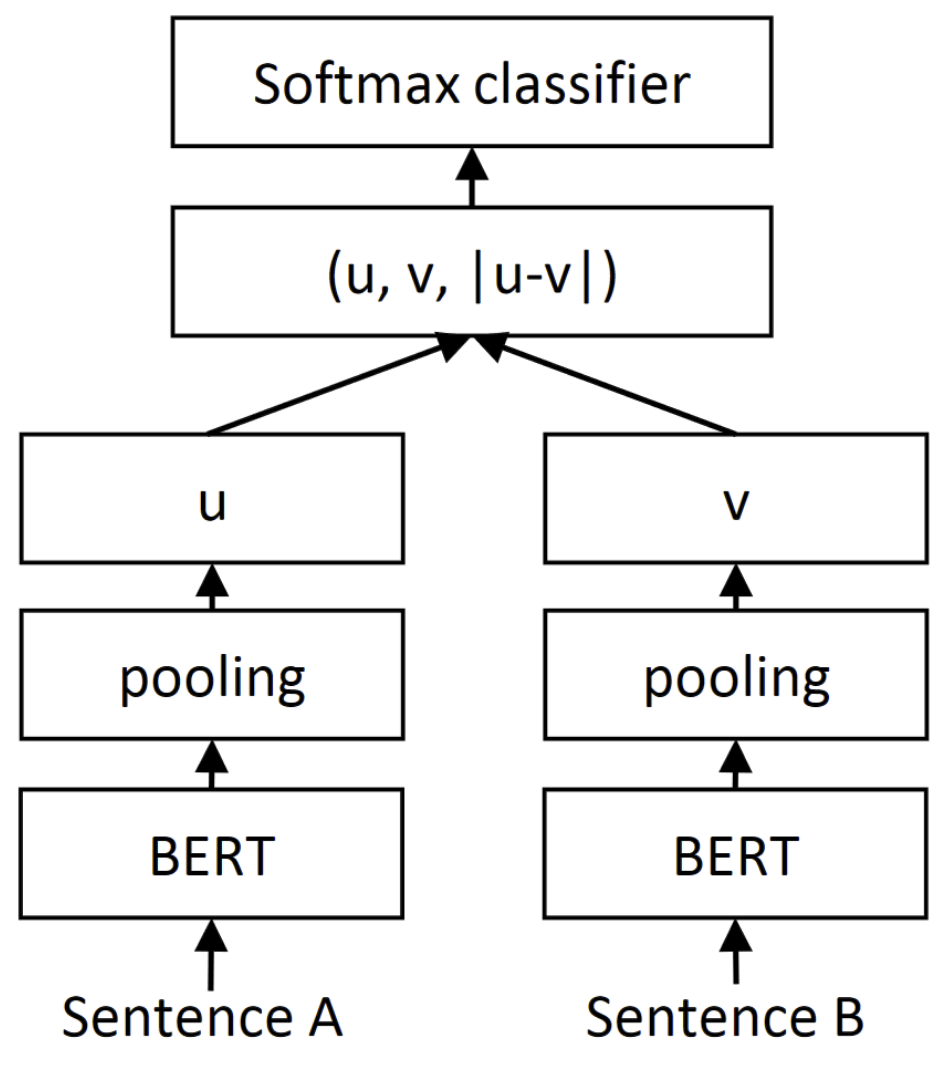
\includegraphics[width=0.3\linewidth]{rys03/sbert.png}
		\caption{Architektura modelu Sentence-BERT\cite{sbert}}
	\end{figure}

	Ze względu na specyfikę potrzebnego korpusu do trenowania modeli SBERT (oznaczone pary zdań) nie istnieją obecnie modele wytrenowane w języku polskim.
	Jednak w roku 2020 ci sami autorzy opracowali metodę przenoszenia wiedzy (ang.\ \emph{transfer learning}) z nauczonego modelu angielskiego na modele wielojęzykowe\cite{sbert_multilingual}.
	


\section{Wektory wypowiedzi}\label{sec:sentences}

  Podział na zdania - trza bo:
  \begin{figure}[ht]
    \begin{minipage}{.75\textwidth}\label{fig:word_count}
      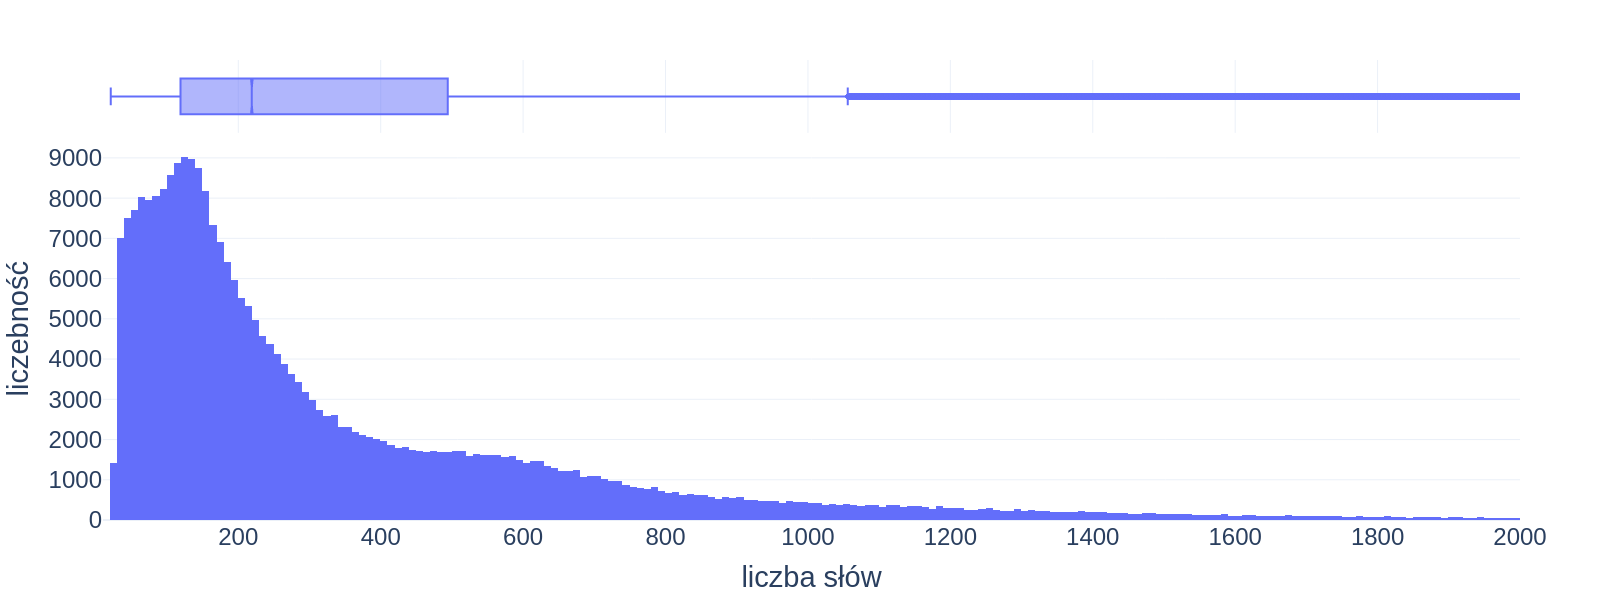
\includegraphics[width=\textwidth]{rys03/word_count.png}
    \end{minipage}%
    \begin{minipage}{.25\textwidth}\label{tab:word_count}
      \small
      \begin{tabularx}{\textwidth}{l|l}
        Min & 21 \\ 
        Q1 & 119 \\ 
        Mediana & 219 \\
        Q3 & 494 \\ 
        Górny wąs & 1056 \\
        Max & 28.546 \\
      \end{tabularx}
    \end{minipage}
    \caption{Dystrybucja długości wypowiedzi (zakres do 2000 słów)}
  \end{figure}